\documentclass{article}
\usepackage{tikz}
\usetikzlibrary{positioning}
\usetikzlibrary{shapes.geometric}
\usetikzlibrary{shapes.symbols}
\usetikzlibrary{shadows}
\usetikzlibrary{arrows}

\pagestyle{empty}

\begin{document}

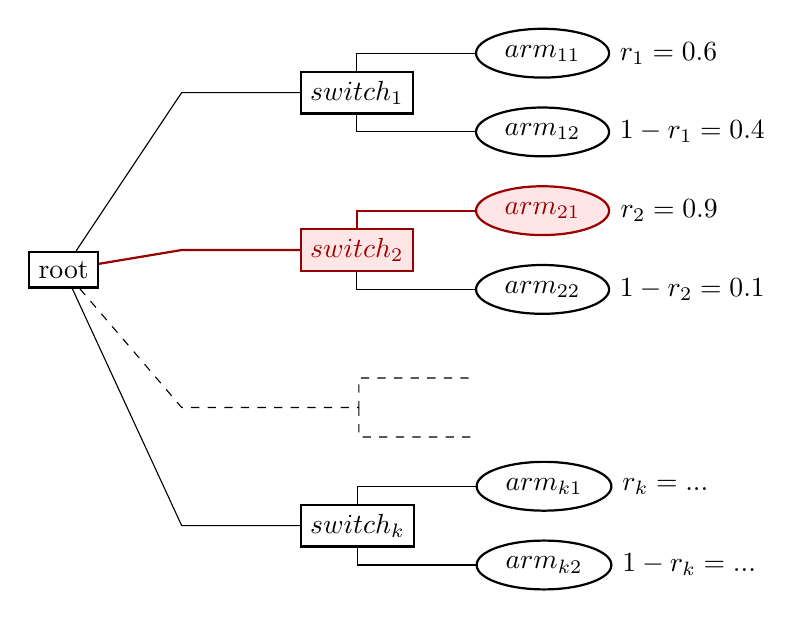
\begin{tikzpicture}
[switch/.style={shape=rectangle,draw,thick,right},
 arm/.style={shape=ellipse,draw,thick,right},
 selected/.style={draw=red!60!black},
 seledge/.style={selected,thick},
 selnode/.style={red!60!black,selected,fill=red!10!white}]

\draw (0,0) node (root) [switch] {root};

\draw (root) -- ++(1.5,2.25) -- ++(1.5, 0)
	node (s1) [switch] {$switch_1$};
\draw (s1) -- ++(0, 0.5) -- ++(1.5, 0)
	node (a11) [arm,label=right:{$r_1=0.6$}] {$arm_{11}$};
\draw (s1) -- ++(0, -0.5) -- ++(1.5, 0)
	node (a12) [arm,label=right:{$1-r_1=0.4$}] {$arm_{12}$};

\draw [seledge] (root) -- ++(1.5,0.25) -- ++(1.5, 0)
	node (s2) [switch,selnode] {$switch_2$};
\draw [seledge] (s2) -- ++(0, 0.5) -- ++(1.5, 0)
	node (a21) [arm,label=right:{$r_2=0.9$},selnode] {$arm_{21}$};
\draw (s2) -- ++(0, -0.5) -- ++(1.5, 0)
	node (a22) [arm,label=right:{$1-r_2=0.1$}] {$arm_{22}$};

\draw [dashed] (root) -- ++(1.5, -1.75) -- ++(2.25, 0)
	-- ++(0, 0.375) -- ++(1.5, 0) ++(-1.5, -0.375) -- ++(0, -0.375) -- ++(1.5, 0);


\draw (root) -- ++(1.5,-3.25) -- ++(1.5, 0)
	node (s3) [switch] {$switch_k$};
\draw (s3) -- ++(0, 0.5) -- ++(1.5, 0)
	node (a31) [arm,label=right:{$r_k=...$}] {$arm_{k1}$};
\draw (s3) -- ++(0, -0.5) -- ++(1.5, 0)
	node (a32) [arm,label=right:{$1-r_k=...$}] {$arm_{k2}$};
\end{tikzpicture}
\end{document}
